\section{7. Eigenvalues and Eigenvectors}
% ***************************************

\subsection{Introduction to eigenvalues and eigenvectors}
% =======================================================

Eigenvector \textbf{u} and eigenvalue $\lambda$ of a square matrix \textbf{A} is a 
of vector and matched scalar value so that
$$\mathbf{Au} = \lambda\mathbf{u}
$$
If you imagine the matrix \textbf{A} as a transformation, \textbf{u} is that vector that transformed
by \textbf{A} is only shrank or extended in length, but it is not rotated or transposed.
The magnitude of extension/shrinkage that \textbf{A} applies to \textbf{u} is the
scalar value $\lambda$, the eigenvalue.

The eigenvalues are found by applying the \textbf{characteristic equation}

$$
det(\mathbf{A - I}\lambda) = \mathbf{0}
$$

Where does the characteristic equation come from? Consider the following re-arragments:

$\mathbf{Au} = \lambda\mathbf{u} \rightarrow$

$\mathbf{Au} = \lambda\mathbf{Iu}$ \emph{multiply by \textbf{I} doesn't change anything}

$\mathbf{Au} - \lambda\mathbf{Iu} = \mathbf{0}$

$(\mathbf{A} - \lambda\mathbf{I})\mathbf{u} = \mathbf{0}$ 

Consider the matrix $\mathbf{A} - \lambda\mathbf{I}$, what value of $\lambda$ makes
this matrix equal to \textbf{0}? Answer, solve $det(\mathbf{A} - \lambda\mathbf{I}) = \mathbf{0}$
for $\lambda$.

\href{http://www.researchgate.net/post/What_is_the_physical_significance_of_eigenvalues_or_eigenvectors_Please_try_to_explain_in_very_simple_language}
{This} is a useful informal description of eigenvalues/vectors:

\emph{If we consider matrix as a transformation then in simple terms eigenvalue is the
strength of that transformation in a particular direction known as eigenvector.}

\subsubsection{Exercise 7.1.1.}
% -----------------------------
Find the eigenvalues and eigenvectors of the matrix
$\mathbf{A} = \left[\begin{matrix}7 & 3\\0 & -4\end{matrix}\right]$.

First find the eigenvalue(s) by setting
$$
det(\mathbf{A - I}\lambda) =
det(\left[\begin{matrix}7 & 3\\0 & -4\end{matrix}\right] - \left[\begin{matrix}\lambda & 0\\0 & \lambda\end{matrix}\right]) =
det(\left[\begin{matrix}- \lambda + 7 & 3\\0 & - \lambda - 4\end{matrix}\right]) =
\lambda^{2} - 3 \lambda - 28 = 0
$$

Solving $\lambda^{2} - 3 \lambda - 28 = 0$ we find $\lambda = -4; \lambda= 7$.

To find the correspondong eigenvectors, substitute each value of $\lambda$ in $\mathbf{Au} = \lambda\mathbf{u}$
and solve for \textbf{u}. For $\lambda= -4$ we have

$$
\mathbf{Au} = \lambda\mathbf{u}; \quad
\left[\begin{matrix}7 & 3\\0 & -4\end{matrix}\right]
\left[\begin{matrix}x_{1}\\x_{2}\end{matrix}\right] = -4 \left[\begin{matrix}x_{1}\\x_{2}\end{matrix}\right]
$$

solved for $x_1$

$$
\left \{ x_{1} : - \frac{3 x_{2}}{11}\right \}
$$

Setting $x_2$ to, say, 1 we obtain the eigenvector $\mathbf{u}_{\lambda= -4}= [-3/11 \quad 1]^T$. \textbf{NB} we could
set $x_2$ to any value, for example $x_2= 11$ and obtain $[-3 \quad 11]^T$. In fact,
there is an infinite number of equivalent eigenvectors for each eigenvalue since
any multiple of \textbf{u}, \emph{i.e.} $k\mathbf{u}$ for $k \neq 0$, is valid.

The point is that matrix \textbf{A} multiplies the vector \textbf{u} by the scalar
$\lambda$, any vector that multiplied by \textbf{A} returns $\lambda\mathbf{u}$ is
an eigenvector of that $\lambda$.

Same for $\lambda= 7$:
$\left[\begin{matrix}7 & 3\\0 & -4\end{matrix}\right]
\left[\begin{matrix}x_{1}\\x_{2}\end{matrix}\right] = -7 \left[\begin{matrix}x_{1}\\x_{2}\end{matrix}\right]
$
the solution for $x_2$ is $\left \{ x_{2} : 0\right \}$ while a value for $x_1$
could be 1, so that $\mathbf{u}_{\lambda= 7} = [1 \quad 0]^T$.

\begin{verbatim}
lamda= symbols('lamda')
A= Matrix(2, 2, [7, 3, 0, -4])

# Find eigenvalue(s)
deta= det(A - eye(A.rows) * lamda)
eigval= solve(deta, lamda)

# Find eigenvectors by sub lambda in A*u=lambda*u
u= Matrix(A.rows, 1, symbols('x1:%s' %(A.rows+1)))
eigvec= Eq(A*u, eigval[0]*u)
s1= solve(eqvec, x1)
eigvec= Eq(A*u, eigval[1]*u)
s2= solve(eqvec, x1)

eigvec= Eq(A*u, eigval[0]*u)
solve(eigveceq, u[0])
\end{verbatim}

\subsubsection{Exercise 7.1.2}
% ----------------------------

Find the general eigenvectors for $\mathbf{A}= \left[\begin{matrix}1 & 0 & 4\\0 & 4 & 0\\3 & 5 & -3\end{matrix}\right]$
given the eigenvalue $\lambda_1= 4$ and $\lambda_2= -5$.

For each given $\lambda$ we need to solve $\mathbf{Au} = \lambda\mathbf{u}$ for
a generic vector $[x\ y\ z]^T$. For $\lambda= 4$ we have solutions $\left \{ x : \frac{4 z}{3}, \quad y : \frac{3 z}{5}\right \}$.
Setting $z= 1$ we obtain $\mathbf{u}_4 = [\frac{4}{3}\ \frac{3}{5}\ 1]^T$ and in general
$\mathbf{u}_4 = k[\frac{4}{3}\ \frac{3}{5}\ 1]^T$. We could use a more convenient
value of $z$, like $z= 15$ so that we obtain $\mathbf{u}_4 = k[20\ 9\ 15]^T$

\begin{verbatim}
x, y, z= symbols('x y z')
A= Matrix([[1, 0, 4], [0, 4, 0], [3, 5, -3]])
u= Matrix(A.rows, 1, [x, y, z])

lamda= 4
evec= Eq(A*u, lamda*u)
sols= solve(evec, [x, y, z])
z1= 1
sols= solve(evec.subs(z, z1), [x, y])
u4= Matrix(A.rows, 1, [sols[x], sols[y], z1])
# Or
z1= 15
sols= solve(evec.subs(z, z1), [x, y])
u4= Matrix(A.rows, 1, [sols[x], sols[y], z1])
\end{verbatim}

\subsubsection{Exercise 7.1.3}
% ----------------------------

Plot the eigenspaces $E_\lambda$ of $\mathbf{A}= \left[\begin{matrix}3 & 1\\1 & 3\end{matrix}\right]$.

This time we use \sympy to find the eigenvectors, which are

$$
\left [ \left ( 2, \quad 1, \quad \left [ \left[\begin{matrix}-1\\1\end{matrix}\right]\right ]\right ),
\quad \left ( 4, \quad 1, \quad \left [ \left[\begin{matrix}1\\1\end{matrix}\right]\right ]\right )\right ]
$$

The output of \sympy \texttt{Matrix.eigenvects()} is a list of tuples, one tuple for eigenvalue. Each
tuple contains: Eigenvalue, multitlicity, eigenvector.

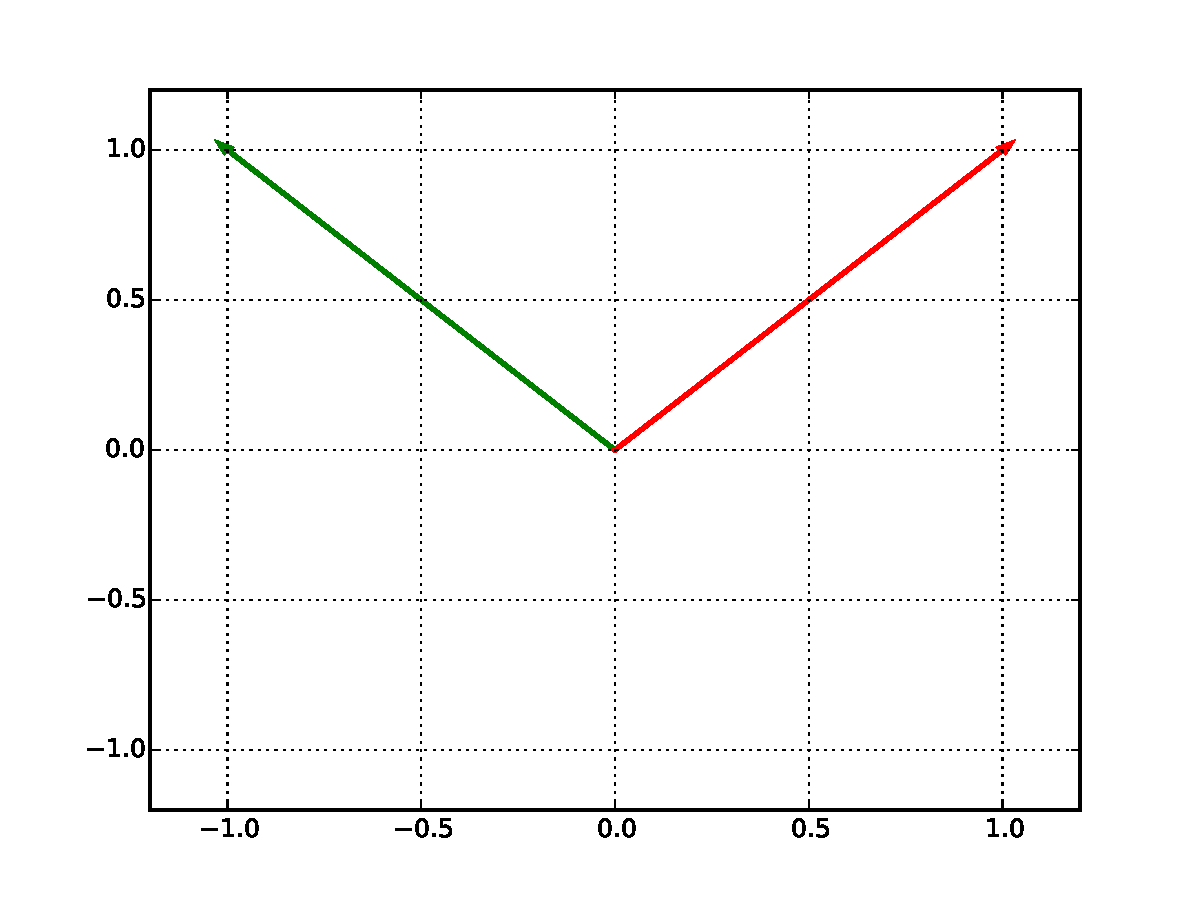
\includegraphics[width=\linewidth]{figs/ex7_1_3.pdf}

\begin{verbatim}
A= Matrix(2, 2, [3, 1, 1, 3])
evecs= A.eigenvects()

plt.subplot()
plt.xlim(-1.2, 1.2)
plt.ylim(-1.2, 1.2)
plt.arrow(0, 0, float(evecs[0][2][0][0]), float(evecs[0][2][0][1]),
    linewidth= 2, color= 'g')
plt.arrow(0, 0, float(evecs[1][2][0][0]), float(evecs[1][2][0][1]),
    linewidth= 2, color= 'r')
plt.grid()
plt.savefig('figs/ex7_1_3.pdf')
plt.close()
\end{verbatim}

\subsubsection{Exercise 7.1.4}
% ----------------------------

What is the effect of multiplying matrix $\mathbf{A}= \left[\begin{matrix}5 & -2\\7 & -4\end{matrix}\right]$ by its eigenvector. Plot the eigenspace
and compute a basis vector for each eigenspace.

Eigenvalues, multiplicity and eigenvectors:

$$
\left [ \left ( -2, \quad 1, \quad \left [ \left[\begin{matrix}\frac{2}{7}\\1\end{matrix}\right]\right ]\right ),
\quad \left ( 3, \quad 1, \quad \left [ \left[\begin{matrix}1\\1\end{matrix}\right]\right ]\right )\right ]
$$

Multiplying (transforming) the eigenvector by the matrix has the same effect as
extending the eigenvector by a factor $\lambda$, there is no change in direction
of the eigenvector. \textit{I.e.} $\mathbf{Au} = \mathbf{\lambda u}$.

The basis for the eigenspace are the eigenvectors
$\mathbf{u} = \left[\begin{matrix}\frac{2}{7}\\1\end{matrix}\right], \quad
\mathbf{v}= \left[\begin{matrix}1\\1\end{matrix}\right]$. Which means \textbf{u}
is the basis vector for $\lambda= -2$ and \textbf{v} is the basis vector for $\lambda= 3$.
They are a basis because every vector in their space can be created by linear combination
of these vector. In fact, every segment sitting on the line $[2/7 \quad 1]^T$ can be
obtained by multiplying $[2/7 \quad 1]^T$ by an appropriate scalar (and the same for any segment sitting
on \textbf{u}).

\begin{verbatim}
A= Matrix(2,2, [5, -2, 7, -4])
evecs= A.eigenvects()
ev= [x[2][0] for x in evecs]

# Au = lambda*u
u= evecs[0][2][0]
lamu= evecs[0][0]
A* u == lamu * u ## True

v= evecs[1][2][0]
lamv= evecs[1][0]
A* v == lamv * v ## True
\end{verbatim}

\subsection{Properties of eigenvalues and eigenvectors}
% =====================================================

\subsubsection{Exercise 7.2.3}
% ----------------------------

The characteristic equation is the characteristic polynomial equated to zero.

The characteristic polynomial ($p(\lambda)$) for a 2x2 matrix \textbf{A} is
$p(\lambda) = det(\mathbf{A} - \lambda \mathbf{I})$ and it is equivalent
to $p(\lambda) = \lambda^2 - tr(\mathbf{A}) \lambda + det(\mathbf{A})$, as shown below.

\begin{verbatim}
a,b,c,d= symbols('a:d', real= True)
lamda= symbols('lambda', real= True)
A= Matrix(2, 2, [a, b, c, d])

charp= lamda**2 - A.trace() * lamda + A.det()
chareq= det(A - lamda * eye(2))
Eq(chareq.expand() - charp.expand()) # True
\end{verbatim}

Note that equality between polynomials is tested after \texttt{expand}ing them to canonical
form. Simply testing \texttt{charp - chareq} will not return 0 as it should. See also
\sympy \href{https://github.com/sympy/sympy/wiki/Faq}{FAQ}

\subsubsection{Exercise 7.2.4}
% ----------------------------

Given \textbf{A} a 2x2 matrix with $tr(\mathbf{A}) = 2a$ and $det(\mathbf{A}) = a^2$,
obtain the eigenvalue $\lambda$. 

Start from the characteristic polynomial $p(\lambda) = \lambda^2 - tr(\mathbf{A})\lambda + det(\mathbf{A})$
and substitute the values $tr(\mathbf{A}) = 2a$ and $det(\mathbf{A}) = a^2$. The resulting
equation $p(\lambda) = a d - b c + \lambda^{2} - \lambda \left(a + d\right)$ is solved
for $\lambda= a$. Therefore given the conditions above an eigenvalue of \textbf{A} is
$a$. Since $a$ is the only solution and the matrix is 2x2, than $a$ has multiplicity 2,
\textit{i.e.} it occurs twice.

\begin{verbatim}
a,b,c,d= symbols('a:d', real= True)
lamda= symbols('lambda', real= True)
A= Matrix(2, 2, [a, b, c, d])

charp= lamda**2 - A.trace() * lamda + A.det()
charp2= charp.subs(A.trace(), 2*a).subs(A.det(), a**2)
ev= solve(charp2, lamda) # [a]
\end{verbatim}

\subsubsection{Exercise 7.2.5}
% ----------------------------

For $\mathbf{A} = \left[\begin{matrix}1 & 0 & 0\\-3 & 1 & 0\\7 & 9 & 1\end{matrix}\right]$
obtain eigenvalues and eigenvectors. Write down a set of basis vectors.

Since this is a triangular matrix, the eigenvalues can be read from the main diagonal.
In this case $\lambda= 1$ with multiplicity 3. Consequently there is only one eigenvector
$\mathbf{v}= [0\ 0\ 1]^T$.

The basis is $\mathbf{x\ y\ z}= [0\ 0\ 1]^T$ which means that the eigenspace for
$\lambda= 1$ is the vertical axis $z$ in 3D space.

\begin{verbatim}
A= Matrix([[1, 0, 0], [-3, 1, 0], [7, 9, 1]])
ev= A.eigenvects()
\end{verbatim}

Note that in triangular matrices only the leading diagonal determines the eigenvalues/vectors.
The generic triangular matrix $\left[\begin{matrix}1 & 0 & 0\\a & 1 & 0\\b & c & 1\end{matrix}\right]$
has the same values as the matrix \textbf{A} above:

\begin{verbatim}
A1= Matrix([[1, 0, 0], [a, 1, 0], [b, c, 1]])
ev1= A.eigenvects() ## Same as above
ev == ev1 # True
\end{verbatim}

Note that if n eigenvalues are distinct then the corresponding eigenvectors are
linearly independent.

\subsection{Diagonalization}
% ==========================

Diagonalization is the process of converting an n x n matrix in a diagonal one. The
values on the diagonal matrix are the eigenvalues of the original matrix. Diagonal
matrices are much easier to work with then full matrices.

The power of matrices, useful in Markov models, is much simplified by means of
diagonalization since $\mathbf{D}^n$ is easy to compute if \textbf{D} is a diagonal
matrix.

Diagonalize \textbf{A} means that:

$$
\mathbf{P^{-1} A P = D} \quad and \quad
\mathbf{A = P D P^{-1}}
$$



That is, there exists a matrix \textbf{P} so that the multiplication above transforms
\textbf{A} into a diagonal matrix \textbf{D}. \textbf{P} is a matrix of eigenvectors
of \textbf{A}:

$$
\mathbf{A^m = P  D^m  P^{-1}}
$$

(that's why diagonalization appears in the chapter about eigenvalues/vectors).

\subsubsection{Exercise 7.3.1}
% ----------------------------

\begin{verbatim}
A= Matrix(2, 2, [1, 0, 0, 2])
evecs= [x[2][0] for x in A.eigenvects()]
P= Matrix(np.column_stack(evecs))
D= P.inv() * A * P
Eq(A, P * D * P.inv())

A= Matrix(2, 2, [2, 2, 1, 3])
evecs= [x[2][0] for x in A.eigenvects()]
P= Matrix(np.column_stack(evecs))
D= P.inv() * A * P
Eq(A, P * D * P.inv())
\end{verbatim}

\subsubsection{Exercise 7.3.2}
% ----------------------------

Find $\mathbf{A}^5$ for $\mathbf{A} = \left[\begin{matrix}2 & 2\\1 & 3\end{matrix}\right]$.

\begin{enumerate}
\item Find the eigenvectors of \textbf{A}. Put them in matrix \textbf{P} by column binding.
\item Get the eigenvalues of \textbf{A}. Put them along the diagonal matrix \textbf{D}.
\item Calculate power of \textbf{A} as $\mathbf{A}^m = \mathbf{PD^mP^{-1}}$ for $m= 5$. 
\end{enumerate}

We use \sympy \texttt{Matrix.eigenvects} to obtain eigenvectors/values.  For \textbf{A}
we have the list of tuples $\left [ \left ( 1, \quad 1, \quad \left [ \left[\begin{matrix}-2\\1\end{matrix}\right]\right ]\right ), \quad \left ( 4, \quad 1, \quad \left [ \left[\begin{matrix}1\\1\end{matrix}\right]\right ]\right )\right ]$.
Each tuple is (eigenvalue, multiplicity, eigenvector).

The matrix of eigenvectors is $\mathbf{P} = \left[\begin{matrix}-2 & 1\\1 & 1\end{matrix}\right]$
and the diagonal matrix of eigenvalues is $\mathbf{D} = \left[\begin{matrix}1 & 0\\0 & 4\end{matrix}\right]$

Now $\mathbf{A}^5$ is easy to compute as $\mathbf{A}^5 = \mathbf{P D^5 P^{-1}} =
\left[\begin{matrix}-2 & 1\\1 & 1\end{matrix}\right]
\left[\begin{matrix}1^5 & 0\\0 & 4^5\end{matrix}\right]
\left[\begin{matrix}- \frac{1}{3} & \frac{1}{3}\\\frac{1}{3} & \frac{2}{3}\end{matrix}\right] =
\left[\begin{matrix}342 & 682\\341 & 683\end{matrix}\right]$

\begin{verbatim}
A= Matrix(2, 2, [2, 2, 1, 3])

def powerMat(A, m):
    """Return the square matrix A to the power of m"""
    # Eigenvectors/values
    ev= A.eigenvects()
    P= Matrix(np.array([x[2][0] for x in ev])).transpose()
    D= diag(*[x[0] for x in ev])
    Am= P * D**Rational(m) * P.inv()
    return Am

A5= powerMat(A, 5)
    
## Check against SymPy
A**5 == A5 ## True
\end{verbatim}

For $\mathbf{A} = \left[\begin{matrix}3 & 0\\4 & 4\end{matrix}\right] ^ {-1/2} =
\left[\begin{matrix}\frac{\sqrt{3}}{3} & 0\\- \frac{4 \sqrt{3}}{3} + 2 & \frac{1}{2}\end{matrix}\right]$

Note the use of \texttt{Rational(-1/2)} required by \sympy to deal with rational
numbers.

\begin{verbatim}
A= Matrix(2, 2, [3, 0, 4, 4])
Am= powerMat(A, -1/2)
A**Rational(-1/2) == Am ## True
\end{verbatim}

\subsubsection{Exercise 7.3.4}
% ----------------------------

Determine whether the following matrices are diagonalizable.

To answer the question consider that:

\begin{itemize}
\item If an $n$ x $n$ matrix has $n$ distinct eigenvalues, than the corresponding
eigenvectors are \emph{linearly independent}.

\item If an $n$ x $n$ matrix has $n$ distinct eigenvalues then the matrix is diagonalizable.
\end{itemize}

Note that in some cases a matrix can be diagonalizable even if doesn't have $n$ distinct eigenvalues
(\emph{I.e.} the above is not an \emph{if and only if} condition).

For the identity matrix $\mathbf{A} = \left[\begin{matrix}1 & 0 & 0\\0 & 1 & 0\\0 & 0 & 1\end{matrix}\right]$
we have one eigenvalue $\lambda = 1$ with multiplicity 3 and eigenvectors
$\left [ \left[\begin{matrix}1\\0\\0\end{matrix}\right], \quad \left[\begin{matrix}0\\1\\0\end{matrix}\right], \quad \left[\begin{matrix}0\\0\\1\end{matrix}\right]\right ]$.

The matrix of eigenvectors therefore is $\mathbf{P} = \left[\begin{matrix}1 & 0 & 0\\0 & 1 & 0\\0 & 0 & 1\end{matrix}\right]$,
and the matrix of eigenvalues $\mathbf{P} = \left[\begin{matrix}1 & 0 & 0\\0 & 1 & 0\\0 & 0 & 1\end{matrix}\right]$.

The identity matrix is therefore diagonalizable even if the distinct eigenvalues is less
than the matrix dimension since $\mathbf{I} = \mathbf{A} = \mathbf{P D P^{-1}}$.

\begin{verbatim}
A= eye(3)
ev= A.eigenvects()
P= Matrix(np.column_stack(ev[0][2])).transpose()
D= diag(*[ev[0][0]]*A.rows)

A == P * D * P.inv() # True
\end{verbatim}

For $\mathbf{A} = \left[\begin{matrix}-1 & 2 & 3\\0 & 2 & 5\\0 & 0 & 8\end{matrix}\right]$
the matrix is triangular and therefore the eigenvalues are on the leading diagonal.
The eigenvalues are distinct and therefore the matrix is diagonalizable.

\begin{verbatim}
A= Matrix([[-1, 2, 3], [0, 2, 5], [0, 0, 8]])
ev= A.eigenvects()
P= Matrix(np.array([x[2][0] for x in ev])).transpose()
D= diag(*[x[0] for x in ev])
A == P * D * P.inv()
\end{verbatim}

\subsection{Diagonalization of Symmetric Matrices}
% ================================================

Some useful definitions and properties:

\begin{itemize}

\item A matrix is symmetric if $\mathbf{A = A^T}$.

\item Symmtric matrices can be diagonalized by an orthogonal matrix. 

\item Orthogonality: Two vectors are orthogonal, \emph{i.e.} their angle is 90$^{\circ}$,
if their inner (dot) product is zero:

$$
\mathbf{u \cdot v} = 0
$$

Note that orthogonality makes sense for vectors of any dimension even if geometrically
vectors of length $>3$ cannot be visualized

\item The distinct eigenvalues of a symmetric matrices have corresponding eigenvectors
which are othogonal. \emph{N.B.} the covariance matrix is symmetric.

For example, matrix $\mathbf{M}= \left[\begin{matrix}-5 & 4 & 2\\4 & -5 & 2\\2 & 2 & -8\end{matrix}\right]$
is symmetric and has the following eigenvalues, multiplicity and eigenvectors
$$\left [ \left ( -9, \quad 2, \quad \left [ \left[\begin{matrix}-1\\1\\0\end{matrix}\right],
\quad \left[\begin{matrix}- \frac{1}{2}\\0\\1\end{matrix}\right]\right ]\right ),
\quad \left ( 0, \quad 1, \quad \left [ \left[\begin{matrix}2\\2\\1\end{matrix}\right]\right ]\right )\right ]$$

Eigenvalue -9 has multiplicity 2 (two eigenvectors), and these are \emph{not} orthogonal.
However, these two eigenvectors are orthogonal to the eigenvector with eigenvalue
0: $\left[\begin{matrix}-1\\1\\0\end{matrix}\right] \cdot \left[\begin{matrix}- \frac{1}{2}\\0\\1\end{matrix}\right]  = 1/2$ and
$\left[\begin{matrix}2\\2\\1\end{matrix}\right] \cdot \left[\begin{matrix}-1\\1\\0\end{matrix}\right] =
\left[\begin{matrix}2\\2\\1\end{matrix}\right] \cdot \left[\begin{matrix}- \frac{1}{2}\\0\\1\end{matrix}\right] = 0$

\begin{verbatim}
M= Matrix([[-5, 4, 2],
           [4, -5, 2],
           [2, 2, -8]])
ev= M.eigenvects()
u= ev[0][2][0]
v= ev[0][2][1]
z= ev[1][2][0]

u.dot(v) == 0 # False
z.dot(u) == 0 # True
z.dot(v) == 0 # True
\end{verbatim}

\item A matrix \textbf{Q} is \textbf{orthogonal} if its column vectors are orthogonal to each other and
of norm 1, \emph{i.e.} they orthonormal.

\item \textbf{Orthogonal diagonalization} of matrix \textbf{A} means the following decomposition

$$
\mathbf{A = Q^{-1}DQ = Q^TDQ}
$$

As before, \textbf{Q} column-binds the normalized eigenvectors of \textbf{A}. \textbf{D}
is a diagonal matrix with the eigenvalues of \textbf{A} along the leading diagonal.

\item Because of the diagonalization $\mathbf{A = Q^{-1}DQ = Q^TDQ}$ symmetric
matrices are easy to diagonalize since we don't need to invert \textbf{Q}, an
expensive operation, we just need to transpose \textbf{Q}.
\end{itemize}

\subsubsection{Exercise 7.4.1}
% ----------------------------

Find and orthogonal matrix \textbf{Q} which diagonalizes the following matrices.

\begin{itemize}
\item Find eigenvectors of \textbf{A}, column-bind them
\end{itemize}

\begin{verbatim}

def normalize(v):
    """Normalize vector v
    """
    vsq= sqrt(sum([x**2 for x in v]))
    return 1 / vsq * v 

def getQD(M):
    """Return a tuple of
    * Matrix of normalized eigenvectors of M column binded
    * Diagonal matrix of eigenvalues of A
    """
    assert M == M.transpose() # Check M is symmetric.
    ev= M.eigenvects()
    eigval_lst= []
    eigvec_lst= []
    for vmv in ev:
        eigvec= vmv[2]
        for v in eigvec:
            # For each eigenvector in this eigenvalue.
            eigval_lst.append(vmv[0])
            vnorm= normalize(v)
            eigvec_lst.append(list(vnorm))
    Q= Matrix(eigvec_lst).transpose()
    assert Q * Q.transpose() == eye(A.rows) # Test Q is orthogonal
    D= diag(*eigval_lst)
    return (Q, D)

A= Matrix(2, 2, [1, 0, 0, 2])
Q,D= getQD(A)
Q.transpose() * A * Q == D # True

# ----

A= Matrix(2, 2, [5, 12, 12, -5])
Q,D= getQD(A)
Q.transpose() * A * Q == D # True

# ----

A= Matrix([[5, sqrt(12)], [sqrt(12), 1]])
Q,D= getQD(A)
Q.transpose() * A * Q == D # True
\end{verbatim}


\subsection{Singular Value Decomposition}
% =======================================

Useful concepts and properties:

\begin{itemize}
\item Eigenvalues/vectors can be obtained only for square matrices, so if \textbf{A}
is not square we can't get eigenvalues/vectors.
\item Good news is $\mathbf{A^TA}$ is square \emph{and} symmetric! This means that
$\mathbf{A^TA}$ can be easily diagonalized.
\item The eigenvalues of $\mathbf{A^TA}$ are either positive or zero.
\end{itemize}

\subsubsection{Exercise 7.5.1}
% ----------------------------

Decompose \textbf{A} so that

$$
\mathbf{A = UDV^T}
$$

\begin{itemize}

\item Singular values of \textbf{A}: The square root of the eigenvalues of $\mathbf{A^TA}$, denoted
$\sigma_1, \sigma_2, \dots, \sigma_n$ with $n$ the number of columns in \textbf{A}.
The eigenvectors corresponding to $\sigma_i$, $\mathbf{v_i}$ give the equation
$$
\mathbf{\sigma_i u_i = Av_i}
$$

$\sigma$s and vectors \textbf{v} should be in order largest to smallest.

\item $\mathbf{U}$ Matrix of vectors normalized $\mathbf{u_i}$ from above.

\item $\mathbf{D}$: Diagonal matrix of singular values of \textbf{A}.

$$
\mathbf{D} = \left[\begin{matrix}\sigma_{1} & 0 & 0\\0 & \sigma_{2} & 0\\0 & 0 & \sigma_{n}\end{matrix}\right]
$$

Take care of the size of \textbf{D}. If \textbf{A} is rectangular with more rows than columns, than the diagonal is filled up with zeros.


\item $\mathbf{V}$: Matrix of eigenvectors of $\mathbf{A^TA}$ of size $n$:

$$
\mathbf{V = (v_1\ v_2 \dots v_n)}
$$

\end{itemize}

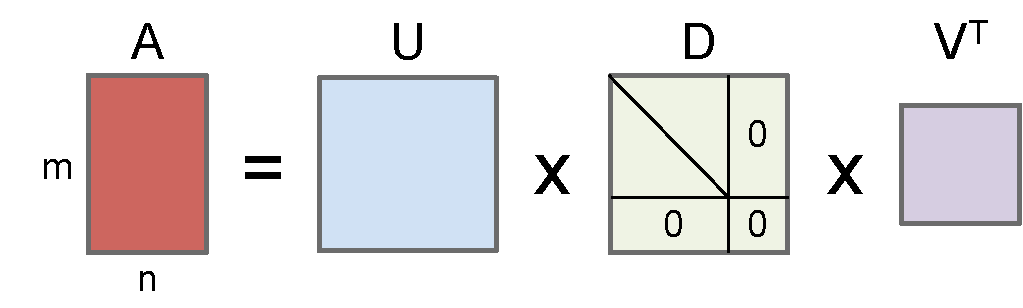
\includegraphics[width=0.7\linewidth]{figs/SVD_UDV.pdf}

For matrix \textbf{A}
$$
\mathbf{A} = \left[\begin{matrix}1 & 0\\0 & 1\\1 & 2\end{matrix}\right]
$$

We have:
$$
\mathbf{A^TA} = \left[\begin{matrix}2 & 2\\2 & 5\end{matrix}\right]
$$

$\sigma$s are $\left [ \sqrt{6}, \quad 1\right ]$ which go in \textbf{D} matrix

$$
\mathbf{D} = \left[\begin{matrix}\sqrt{6} & 0\\0 & 1\end{matrix}\right]
$$

Matrix \textbf{U} has the \textbf{u} vectors:

$$
\mathbf{U} = \left[\begin{matrix}\frac{\sqrt{30}}{30} & - \frac{2 \sqrt{5}}{5}\\\frac{\sqrt{30}}{15} & \frac{\sqrt{5}}{5}\\\frac{\sqrt{30}}{6} & 0\end{matrix}\right]
$$

Finally, \textbf{V}:

$$
\mathbf{V} = \left[\begin{matrix}\frac{\sqrt{5}}{5} & - \frac{2 \sqrt{5}}{5}\\\frac{2 \sqrt{5}}{5} & \frac{\sqrt{5}}{5}\end{matrix}\right]
$$

Check $\mathbf{A = UDV^T}$.

\emph{This code is not always correct!}

\begin{verbatim}
A= Matrix([[1, 0], [0, 1], [1, 2]])

# Singular values and Matrix D
AtA= A.T * A
svv= sorted(AtA.eigenvects(), key= lambda x: x[0], reverse= True)
sigmas= [sqrt(x[0]) for x in svv]
atavecs= [x[2][0] for x in svv]
atavecs= [normalize(x) for x in atavecs]
          
U= []
D= []
V= []
for v, s in zip(atavecs, sigmas):
    if s == 0:
        continue
    u_i= A*v / s    # u_1 = A * v_i
    U.append(u_i)
    D.append(s)
    V.append(v)
U= Matrix(np.array(U)).T
D= diag(*D)
V= Matrix(np.array(V)).T

# Check decomposition
A == U * D * V.T
\end{verbatim}

\subsubsection{Interpreting the decompostion}
% -------------------------------------------

Since a matrix \textbf{A} can be thought of a transformation, we can ask the question
of what operations lead to such a transformation.

The SVD decomposes \textbf{A} into three simple transformations
\footnote{From \href{http://en.wikipedia.org/wiki/Singular_value_decomposition}{Wikipedia Singular value decomposition}}:

\begin{itemize}
    \item An initial rotation $\mathbf{V^T}$. \textbf{V} is a symmetric matrix, so its action is to rotate.
    \item A scaling \textbf{D} along the coordinate axes. \textbf{D} is diagonal, so its action is to stretch or shrink, without rotating or shearing.
    \item A final rotation \textbf{U}. The lengths $\sigma_1$ and $\sigma_2$ of the semi-axes are the singular values of M.
\end{itemize}

See also the applet at \href{http://mathforum.org/mathimages/index.php/Transformation_Matrix}{Transformation Matrix} for some effects of matrix transformation 